\chapter{Практическое применение}
\section {Анализ требований}

Очевидно, что ни одна серийная установка быстрого прототипирования не обладает техническими возможностями для реализации предлагаемого подхода на практике. Возможность такого подхода должна быть заложена при разработке устройства. При этом должна использоваться система, отличная от методик, применяемых при проектировании пятикоординатных фрезерных станков, так как эти устройства реализуют разные технологии. В целом к установке быстрого прототпирования может быть выдвинут ряд требований:

\begin{itemize}
\item[$-$] организация возможности перемещения рабочего модуля в, как минимум, пяти координатах;
\item[$-$] возможность упрощения составления УП при загрузке модели, другими словами, задание положения рабочего модуля при помощи элементарных манипуляций;
\item[$-$] возможность построения модели при помощи разных методик;
\item[$-$] минимальные отклонения от стандарта FDM-устройств.
\end{itemize}

Однако, такой подход обладает рядом ограничений при построении модели и проектировании устройства, которые тоже необходимо учитывать. К этим ограничениям относятся:

\begin{itemize}
\item[$-$] физические характеристики расплавленного материала, позволяющие строить лишь верхнюю половину описываемой сферической поверхности;
\item[$-$] размеры устройства, которые должны учитывать все варианты перемещения рабочего модуля, а также размеры самого рабочего модуля;
\item[$-$] максимальный размер получаемой модели, напрямую исходящий из размеров устройства;
\end{itemize}

Таким образом, реализуемое устройство при первичном проектировании должно отвечать всем вышеперечисленным требованиям.

Рассматривая рынок технических устройств можно сказать, что наиболее близкой к требованиям является платформа Стюарта.

\section {Концепция установки}

{\bf Платформа Стюарта} или платформа Гью–Стюарта - это вид параллельного манипулятора, состоящего из верхнего и нижнего оснований, соединённых между собой шестью приводами-стойками при помощи шарнирных соединений. Приводы могут быть разного устройства, но чаще всего они являются пневматическими или жидкостными. Расстановка приводов такова, что верхнее основание может как перемещаться параллельно нижнему, так и наклоняться на небольшие углы. Можно сказать, что данная установка как твёрдое тело обладает шестью степенями свободы, то есть, способна совершать три поступательных и три вращательных перемещения. Внешний вид платформы Гью–Стюарта представлен на рисунке \ref{f:pic7}\,\cite{stewart0}.

\begin{figure} [h]
	\centering
	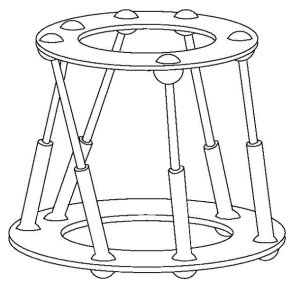
\includegraphics[width=0.5\textwidth]{3-1}
	\caption{Платформа Гью–Стюарта}
	\label{f:pic7}
\end{figure}

\begin{figure} [h]
	\centering
	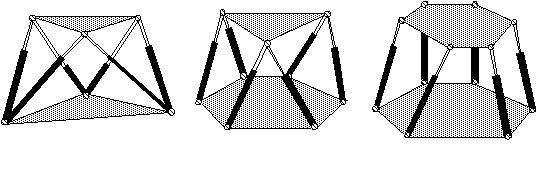
\includegraphics[width=0.8\textwidth]{3-2}
	\caption{Виды платформы Гью–Стюарта}
	\label{f:pic8}
\end{figure}

Разновидностей платформ Стюарта бывает несколько, в зависимости от расположения стоек (рисунок \ref{f:pic8}). Стойки могут быть установлены как по контуру оснований, так и октаэдрально, что даёт разную жёсткость и разную кинематику. Применение данное устройство нашло в самых разных сферах, таких как станкостроение, ортопедическая хирургия, подводные исследования, учебные тренажёры для водителей грузовиков и многих других.

Тем не менее, рассматривая платформу Гью–Стюарта в качестве основы установки быстрого прототипирования, можно отметить некоторые недостатки, которые не позволяют использовать устройство и требуют внесения изменений в конструкцию.

\begin{itemize}
\item[$-$] классическая конструкция не позволяет осуществлять наклоны верхнего основания на достаточно большие углы;
\item[$-$] применение как пневматических, так и гидравлических приводов требует составления системы дифференциальных уравнений динамики и решения обратной кинематической задачи \cite{stewart1};
\item[$-$] использование больших энергозатрат в приводах.
\end{itemize}

При проектировании устройства есть два пути применения механизма: оснастить подвижностью экструдер с соплом либо стол. Подвижность экструдера ограничена токопроводящим оборудованием и каналом подачи материала, который должен быть достаточно гибким, однако сам модуль легче и им проще оперировать. Подвижность стола предполагает наличие более мощных приводов, так как стол обладает большей массой, и наличия некоторого крепежа для модели во избежание падения. Однако, грамотная организация модуля стола позволит уменьшить габариты устройства.

Таким образом, был сделан выбор в пользу первого варианта и, ориентируясь на вышеизложенные проблемы, концепция устроства опирается на механизм платформы, но в конструкции учтены следующие поправки:

\begin{itemize}
\item[$-$] рабочее основание переориентированы с верхнего на нижнее, так как конструкция 3D-принтера подразумевает ориентировку сопла <<вниз>>;
\item[$-$] замена пневматических приводов на шаговые элетроприводы;
\item[$-$] увеличение длины приводных стоек с одновременным уменьшением рабочего основания.
\end{itemize}

Эскизы, отображающий примерный внешний вид устройства, выполненный в 3D-редакторе, представлен на рисунке \ref{f:pic9}. В основе устройства лежит шестиугольная рама на стойках в виде корзины 1, внутри которой располагаются рабочий модуль 2 и стол 3. Рабочий модуль, состоящий из экструдера и сопла, смонтирован на нижнем основании и <<подвешен>> на системе из шести элетроприводов-стоек 4. Электроприводы соединены попарно и располагаются с трёх сторон, каждый из приводов вместе со смежным приводом из другой пары подходят к одной из вершин рабочего основания, выполненного в виде треугольника. Со стороны рамы приводы установлены на двойном шарнире 5 с применением подшипников и ориентированы под углом в 45 градусов к плоскости нижнего основания. Таким образом осуществляется б\'ольшая подвижность рабочего модуля. Канал подачи материала подходит к экструдеру сверху. Стол круглой формы закреплён непосредственно под рабочим основанием и обладает возможностью вертикального перемещения приводом либо, как в данном случае, системой зажимов 6.

Более подробные эскизы находятся в приложении 3.

\begin{figure} [h]
	\centering
	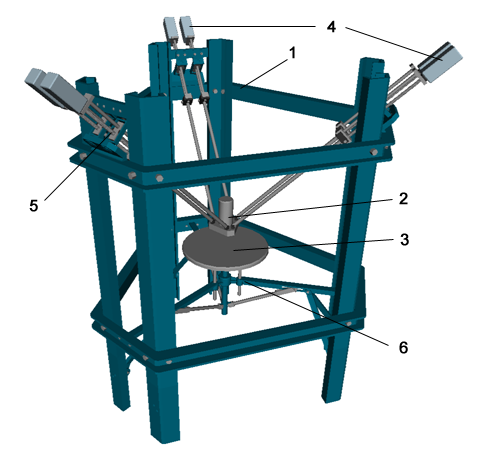
\includegraphics[width=0.6\textwidth]{3-3}
	\caption{Внешний вид установки быстрого прототипирования}
	\label{f:pic9}
\end{figure}

\section {Возможности применения подхода на практике}

Очевидно, что данная методика обладает большим спектром возможностей в производстве моделей и позволяет получать более точные модели. При шести степенях свободы становится возможным манипулировать рабочим модулем в гораздо более обширных пределах. Вот некоторые из возможностей применения:

\begin{itemize}
\item[$-$] получение моделей неоптических линз и других тел вращения с меньшей <<ступенчатостью>> поверхности, и, соответственно, с меньшим временем последующей доработки;
\item[$-$] получение моделей с повышенными прочностными характеристиками за счёт б\'ольшей площади соприкосновения слоёв и их формы;
\item[$-$] получение моделей с совмещением методик построения, другими словами, часть модели может быть выполнена плоскими слоями, часть — криволинейными;
\item[$-$] возможность адаптации CAM-системы к методике построения на основе анализа загруженной модели.
\end{itemize} 
